\documentclass[10pt, fleqn, a4paper]{article}
%% \documentclass[11pt,draftcls,onecolumn]{IEEEtran}

\usepackage[left=2cm,right=2cm,top=1cm,bottom=2cm]{geometry}
\usepackage[utf8]{inputenc}
\usepackage{amsmath,amssymb,amsfonts}
\usepackage{graphicx}
\graphicspath{{../Figures/}}
\usepackage{hyperref}
\usepackage{xspace}
\usepackage{enumitem}
\usepackage{ulem}
\usepackage{cancel}
\usepackage{verbatim}
\usepackage{rotating}
\usepackage{array}
\usepackage{multirow}
\usepackage{color}
\usepackage[french]{babel}
\frenchbsetup{StandardItemLabels}
\usepackage{comment}
\usepackage{eurosym}
\usepackage{xfrac}
\usepackage{manfnt}
\usepackage{pifont}
\usepackage{tcolorbox}
\usepackage{textcomp}

\newcommand\prevyear{\advance\year by -1 \the\year\advance\year by 1}
\newcommand\nextyear{\advance\year by 1 \the\year\advance\year by -1}

% Empty definitions for further redefinitions via \renewcommand:
\newcommand{\Temp}{}
%% Abbreviations communes
\newcommand{\cf}{\emph{cf.}\xspace}
\newcommand{\eg}{\emph{e.g.}\xspace}
\newcommand{\ie}{\emph{i.e.}\xspace}
\newcommand{\etc}{\emph{etc.}\xspace}
\newcommand{\codeblocks}{Code$::$Blocks\xspace}

\newcommand{\touche}[1]{\textnormal{\texttt{\textquotesingle #1\textquotesingle}}}

\newenvironment{algorithme}
{
\begingroup

\footnotesize

\hrulefill

}
{

\hrulefill

\endgroup
}

\definecolor{green}{rgb}{0.0,0.5,0.0}
\definecolor{dred}{rgb}{0.75,0.0,0.0}
\definecolor{purple}{rgb}{0.75,0.0,0.75}
\definecolor{dblue}{rgb}{0.0,0.0,0.75}
\definecolor{dyellow}{rgb}{1.0,0.5,0.0}
\definecolor{orange}{rgb}{1.0,0.5,0.0}
\definecolor{redCM}{rgb}{1.0,0.25,0.25}
\definecolor{blueTD}{rgb}{0.25,0.75,1.0}
\definecolor{greenTP}{rgb}{0.1,0.75,0.5}
\definecolor{lightgreen}{rgb}{0.25,1.0,0.75}
\definecolor{mygray}{gray}{0.45}
\definecolor{redC1}{rgb}{1.0,0.25,0.25}
\definecolor{greenC2}{rgb}{0.0,0.75,0.0}
\definecolor{yellowPORTFOLIO}{rgb}{0.75,1.0,0.0}

\newtcbox{\cboxgenerale}{colback=orange,boxrule=1pt,arc=5pt,
  boxsep=0pt,left=3pt,right=3pt,top=3pt,bottom=3pt}

\newtcbox{\cboxconcevoir}{colback=redC1,boxrule=1pt,arc=5pt,
  boxsep=0pt,left=3pt,right=3pt,top=3pt,bottom=3pt}
  
\newtcbox{\cboxverifier}{colback=greenC2,boxrule=1pt,arc=5pt,
  boxsep=0pt,left=3pt,right=3pt,top=3pt,bottom=3pt}
  
\newtcbox{\cboxportfolio}{colback=yellowPORTFOLIO,boxrule=1pt,arc=5pt,
  boxsep=0pt,left=3pt,right=3pt,top=3pt,bottom=3pt}
  
\newtcbox{\cboxjalon}{colback=orange,boxrule=1pt,arc=5pt,
  boxsep=0pt,left=3pt,right=3pt,top=3pt,bottom=3pt}

\newcommand{\itemcolor}[1]{% Update list item colour
  \renewcommand{\makelabel}[1]{\color{#1}\hfil ##1}}
  
\newcommand{\bfcolor}[2]{\textcolor{#1}{\textbf{#2}}}

\newcommand{\itcolor}[2]{\textcolor{#1}{\textit{#2}}}

\newcommand{\trace}{\fbox{\colorbox{orange}{TRACE}}\xspace}

\newsavebox{\mytextbox}
\newcommand\myframecolor{}
\newcommand\mybgcolor{}
\newenvironment{mycolorbox}[2]
{
\def\myframecolor{#1}
\def\mybgcolor{#2}
\begingroup
\begin{lrbox}{\mytextbox}
\begin{minipage}[t]{\textwidth}
}
{
\end{minipage}\end{lrbox}
\fcolorbox{\myframecolor}{\mybgcolor}{\usebox{\mytextbox}}
\endgroup
}

\def\ESPACEINFO1{\href{https://claroline-connect.univ-st-etienne.fr/web/app.php/workspaces/41547/open?toolName=home}{\bfcolor{orange}{IUTSEGEII\_S1\_M1103\_INFO1}}}

% Uncomment to compile doc with corrections
%\renewenvironment{comment}{}{}

\parindent=0cm

\newcounter{quest}

\begin{document}

\begin{minipage}[l]{\textwidth}
\begin{center}

\includegraphics[width=0.2\textwidth]{logoIUT} \\
\large IUT, Université Jean Monnet, Saint-Étienne \\
\vspace{0.5cm}
\huge \bf{SAé 2 Info2 : Projet d'Algorithmique et Programmation informatique} \\
\vspace{0.2cm}
\Large Année \prevyear-\the\year \\ %-\nextyear \\
\vspace{0.5cm}
\large Fabien Momey, Bruno Bernard, Paul Grandamme, Franck Gérossier, Vincent Grosso, Cyril Mauclair, Thierry Lagniet \\
\end{center}
\end{minipage}

\vspace{0.5cm}

\fbox{\begin{minipage}[l]{\textwidth}
{\bf \underline{INTRODUCTION~:}}

\vspace{1mm}
Cette \bfcolor{greenTP}{Situation d'Apprentissage Évaluée (SAé)} va vous permettre de mettre en œuvre vos \bfcolor{orange}{compétences en programmation informatique} au travers de l'élaboration d'un \bfcolor{orange}{projet complet de réalisation d'une application en C++}, en \bfcolor{redCM}{autonomie} et par \bfcolor{redCM}{groupes de 4 à 5 étudiants}.

Cette SAé sera \bfcolor{redCM}{évaluée}. Un \bfcolor{redCM}{suivi régulier} sera mis en place par l'équipe d'enseignants évaluateurs, avec des \bfcolor{redCM}{jalons à respecter} pour le rendu de certains \bfcolor{redCM}{livrables} (rapport, codes, etc.), puis un \bfcolor{redCM}{rendu final}.
\end{minipage}}

\vspace{0.5cm}

\fbox{\begin{minipage}[l]{\textwidth}
{\bf \underline{PRÉREQUIS \& RESSOURCES À DISPOSITION~:}}

Les connaissances nécessaires pour ce projet ont été acquises tout au long du semestre 1 et en début de semestre 2 notamment lors de vos apprentissages dans les ressources \bfcolor{orange}{INFO1/INFO2} mais aussi dans d'autres ressources telles que \bfcolor{orange}{AUTO1/AUTO2}, ainsi qu'en \bfcolor{orange}{SAé ER}.

Ce \bfcolor{greenTP}{PROJET} étant essentiellement basé sur les acquis du \bfcolor{orange}{module INFO1} du premier semestre, vous aurez à disposition toutes les \bfcolor{orange}{ressources} associées sur \ESPACEINFO1. Un onglet \bfcolor{blue}{SAé2 Info2 - Ressources pour le projet d'informatique} a également été créé sur \ESPACEINFO1 dans lequel vous retrouverez le \bfcolor{greenTP}{présent document} ainsi que des \bfcolor{greenTP}{ressources dédiées} \itcolor{greenTP}{(à consulter régulièrement)}.

\vspace{2mm}
{\bf \underline{\textit{Résumé des notions à maîtriser}~:}}
\begin{itemize}
\item[$\looparrowright$] \bfcolor{orange}{Connaissances techniques :}
\begin{itemize}
\item[\ding{223}] \colorbox{yellow}{\bfcolor{orange}{Bases d'algorithmique et programmation informatique.}}
\item[\ding{223}] Variables, types, structures de contrôle (conditions, boucles).
\item[\ding{223}] Tableaux, \colorbox{yellow}{\bfcolor{orange}{structures}}, \colorbox{yellow}{\bfcolor{orange}{pointeurs}}.
\item[\ding{223}] \colorbox{yellow}{\bfcolor{orange}{Fonctions}}~: appel de fonctions, définition de fonctions, notion de \bfcolor{orange}{passage par valeur (entrées en \og{}lecture seule\fg{} E)} et \bfcolor{orange}{passage par adresse (entrées/sorties en \og{}lecture/écriture\fg{} E/S)}.
\item[\ding{223}] \bfcolor{orange}{\textit{Allocation dynamique de mémoire.}}
\end{itemize}
\item[$\looparrowright$] \bfcolor{redC1}{Mise en œuvre d'une solution algorithmique complète exploitant ces connaissances.}
\item[$\looparrowright$] \bfcolor{redC1}{Implémentation d'une solution algorithmique complète dans un langage de programmation (C++).}
\item[$\looparrowright$] Structure d’un programme informatique :
\begin{itemize}
\item[\ding{223}] fichier source principal "\texttt{main.cpp}".
\item[\ding{223}] fichiers d'en-tête "\texttt{.h}" : prototypes des fonctions et déclaration des structures.
\item[\ding{223}] fichiers sources "\texttt{.cpp}" : définition des fonctions.
\end{itemize}
\item[$\looparrowright$] Écriture du code et compilation dans un environnement de développement intégré (IDE) :
\begin{itemize}
\item[\ding{223}] Code$::$Blocks.
\end{itemize}
\item[$\looparrowright$] \bfcolor{greenC2}{Vérification du code} à l'aide de \bfcolor{greenC2}{procédures de test} et \bfcolor{greenC2}{débogage}.
\end{itemize}
\end{minipage}}

\vspace{0.5cm}

\fbox{\begin{minipage}[l]{\textwidth}
{\bf \underline{COMPÉTENCES \& APPRENTISSAGES CRITIQUES MIS EN JEU~:}}

\begin{center}
\cboxconcevoir{C1-N1-CONCEVOIR}
\end{center}

\cboxconcevoir{\textit{C1-N1-AC1 - Produire une analyse fonctionnelle d'un système simple}}

\begin{itemize}
\item[\ding{223}] Pour toutes les étapes de ce projet, vous devrez proposer une solution algorithmique complète et détaillée (découpage fonctionnel, algorithme principal, procédures de test), indépendamment du langage de programmation choisi, qui respecte les contraintes imposées dans le cahier des charges.
\end{itemize}

\cboxconcevoir{\textit{C1-N1-AC2 - Réaliser un prototype pour des solutions techniques matériel ou logiciel}}

\begin{itemize}
\item[\ding{223}] Vous devrez ensuite implémenter dans une application console C++ chaque étape du projet, en traduisant fidèlement la solution algorithmique élaborée.
\end{itemize}

\cboxconcevoir{\textit{C1-N1-AC3 - Rédiger un dossier de fabrication à partir d'un dossier de conception}}

\begin{itemize}
\item[\ding{223}] Vous devrez rédiger une \bfcolor{redCM}{documentation complète} de votre programme, sous forme algorithmique et illustrée par des exemples issues de votre prototypage en C++. \bfcolor{redCM}{Ce rapport doit pouvoir servir de référence à un programmeur tierce qui souhaiterait implémenter votre solution dans un autre langage de programmation}.
\item[\ding{223}] Concernant votre programme C++, ce dernier devra aussi être \bfcolor{redCM}{rigoureusement commenté}, et notamment toutes les fonctions avec leurs \textbf{\{ Rôle, Entrées, Entrées/Sorties, Sortie \}} clairement définis.
\end{itemize}

\begin{center}
\cboxverifier{C2-N1\textcolor{yellow}{(N3)}-VERIFIER}
\end{center}

\cboxverifier{\textit{C2-N1-AC1 - Appliquer une procédure d’essai}}

\begin{itemize}
\item[\ding{223}] Pour chaque étape du projet, lors de la phase de conception algorithmique et d'implémentation, vous devez réfléchir à une batterie de tests unitaires à mettre en place - \textbf{sous forme de procédures à implémenter ou à réaliser avec l'outil \bfcolor{greenC2}{débogueur} par exemple} - pour valider chaque élément de votre solution (programme principal, fonctions, structures, etc.). \bfcolor{redCM}{Toutes les procédures de test devront être rigoureusement décrites et documentées dans votre rapport. Si ce sont des procédures de test implémentées, elles devront être intégrées au code (dans une librairie dédiée par exemple) et rigoureusement commentées}.
\end{itemize}

\cboxverifier{\textit{C2-N1-AC2 - Identifier un dysfonctionnement}}

\begin{itemize}
\item[\ding{223}] L'application des procédures d'essai que vous aurez définies doivent vous permettre de vérifier le bon fonctionnement de votre programme et d'identifier des dysfonctionnements éventuels.
\end{itemize}

\cboxverifier{\textit{C2-N1-AC3 - Décrire les effets d’un dysfonctionnement}}

\begin{itemize}
\item[\ding{223}] En cas d'identification d'un dysfonctionnement, vous devrez garder trace de vos tests et analyses en rédigeant une petite description dans votre \colorbox{yellowPORTFOLIO}{journal de bord} (cf. partie \colorbox{yellowPORTFOLIO}{PORTFOLIO} ci-dessous).
\end{itemize}

\cboxverifier{\color{yellow}\textit{C2-N3-AC2 - Proposer une solution corrective à un dysfonctionnement}}

\begin{itemize}
\item[\ding{223}] Bien entendu, tout dysfonctionnement de votre programme devra être corrigé et l'application de votre procédure d'essai devra permettre de valider la modification. Cette dernière sera également notifiée dans votre \colorbox{yellowPORTFOLIO}{journal de bord}.
\end{itemize}
\end{minipage}}

\vspace{0.5cm}

\fbox{\begin{minipage}[l]{\textwidth}
{\bf \underline{SUIVI \& GESTION DE VOTRE PROJET~:}}

\begin{center}
\cboxportfolio{PORTFOLIO D'APPRENTISSAGE ET D'ÉVALUATION}
\end{center}

\begin{itemize}
\item[\ding{223}] Parallèlement au \bfcolor{redCM}{dossier de documentation}, vous devrez, en fin de projet, également rédiger un \colorbox{yellowPORTFOLIO}{compte-rendu de projet \underline{personnel}} relatant votre gestion de ce dernier en équipe et analysant, avec un regard critique, votre expérience afin d'auto-évaluer vos acquis dans chaque compétence/apprentissage critique qui auront été travaillés. Ce compte-rendu permettra d'alimenter votre \colorbox{yellowPORTFOLIO}{Portfolio d'apprentissage et d'évaluation} qui rentrera en ligne de compte dans l'évaluation de cette \bfcolor{greenTP}{SAé}.
\item[\ding{223}] Pour faciliter la rédaction de ce compte-rendu, nous vous demandons de tenir, tout au long de votre travail sur le projet, un \colorbox{yellowPORTFOLIO}{journal de bord \underline{personnel}} dans lequel vous pourrez consigner toutes vos actions, résultats et remarques \og{}au jour le jour\fg{}. \bfcolor{redCM}{Ce journal de bord servira de document de suivi pour les enseignants évaluateurs et pourra vous être demandé aux différents jalons.}
\end{itemize}

\end{minipage}}

\vspace{0.5cm}

\fbox{\begin{minipage}[l]{\textwidth}
{\bf \underline{JALONS \& LIVRABLES~:}}

Tout au long de l'élaboration des phases du projet, un certain nombre de jalons seront à respecter, avec des dates fixées et des livrables à fournir (codes, journaux de bord, état de la documentation). \bfcolor{redCM}{Ces livrables seront à déposer sur \ESPACEINFO1 dans l'onglet dédié \colorbox{yellow}{\color{red}SAé2 Info2 - Livrables pour le projet d'informatique}}. 

Les jalons sont indiqués par le cartouche suivant à la fin des phases concernées~:

\begin{center}
\cboxjalon{\bf Jalon \& Livrable n$^{\circ}$\textit{i}}
\end{center}

\bfcolor{redCM}{Guettez ces indicateurs dans le sujet du projet, tous les détails y sont donnés.}

Chacun de ces jalons sera évalué par les enseignants-évaluateurs, et des entrevues pourront être prévues.
\bfcolor{redCM}{Voici les dates butoires à respecter (les espace de dépôt sur Claroline Connect seront ouverts ces jours)~:}

\cboxjalon{\bf Jalon \& Livrable n$^{\circ}$1 $\Rightarrow$ 01/04/2022}

\cboxjalon{\bf Jalon \& Livrable n$^{\circ}$2 $\Rightarrow$ 15/04/2022}

\cboxjalon{\bf Jalon \& Livrable n$^{\circ}$3 $\Rightarrow$ 06/05/2022}

\cboxjalon{\bf Jalon \& Livrable n$^{\circ}$4 $\Rightarrow$ 24/05/2022}

\cboxjalon{\bf Jalon \& Livrable n$^{\circ}$5 $\Rightarrow$ 10/06/2022}

\end{minipage}}

\section*{\underline{Sujet du projet - le cahier des charges}}

Dans ce projet, vous allez créer un \bfcolor{greenTP}{application informatique en C++} qui va vous permettre de réaliser un "jeu" simulant une bataille de vaisseaux spatiaux. À terme, l'objectif est de créer un système de combat au tour par tour entre 2 flottes (2 joueurs) composées de plusieurs vaisseaux, pouvant être de types différents. Le combat prendra fin lorsque l'une des 2 flottes est totalement détruite.

Pour mener à bien ce projet, nous avons décomposé sa réalisation \bfcolor{greenTP}{en différentes phases}, à valider au fur et à mesure par des procédures d'essai, pour élaborer petit à petit les éléments du jeu et la mécanique des combats de vaisseaux.

\bfcolor{orange}{Le moteur de l'application à réaliser sera essentiellement basé sur l'utilisation de \colorbox{yellow}{structures} pour \og{}modéliser\fg{} le type \texttt{vaisseau} comme un conteneur englobant un certain nombre de caractéristiques, ainsi que la définition de \colorbox{yellow}{librairies de fonctions} dédiées à manipuler des instances de ces vaisseaux.}

\itcolor{greenTP}{\underline{Nota bene :} le "jeu" que vous allez coder est rudimentaire puisqu'il s'agira d'une simple \textbf{application console} (comme tous nos programmes habituels). L'objectif n'est pas de coder \bfcolor{greenTP}{STARWARS\textsuperscript{TM}~:~Squadrons (Electronic Arts Inc.)}. Néanmoins, ce contexte vous offre la possibilité de mettre en application vos apprentissages en programmation informatique au travers d'un thème que l'on espère assez ludique. Profitez-en pour laisser parler votre imagination sans négliger la rigueur imposée par la finalité de ce travail.}

\subsection*{Avant-propos : organisation du travail de groupe}

Au début de chaque nouvelle phase, nous vous suggérons de réfléchir en commun à la solution que vous élaborerez, puis de vous répartir les différentes tâches à réaliser~:
\begin{itemize}
\item[$\looparrowright$] \colorbox{redC1}{C1-N1-AC1} Élaboration des algorithmes.
\item[$\looparrowright$] \colorbox{redC1}{C1-N1-AC2} Implémentation de la solution.
\item[$\looparrowright$] \colorbox{redC1}{C1-N1-AC3} Rédaction de la documentation.
\item[$\looparrowright$] \colorbox{greenC2}{C1-N1-AC1} Élaboration et réalisation des procédures d'essai.
\item[$\looparrowright$] \colorbox{greenC2}{C1-N1-AC2\&AC3 | C1-N3-AC2} Identification et description des dysfonctionnements, puis et débogage et correction.
\end{itemize}

Bien entendu, certaines tâches se recouvrent et peuvent être traitées par les mêmes membres du groupe. Attention également, d'autres tâches sont \og{}asynchrones\fg{} et vont requérir que d'autres aient d'abord achevé leur propre tâche. \bfcolor{redCM}{Pensez à organiser un système efficace de partage de codes et de documents afin que chaque membre du groupe puisse avoir accès aux développements du projet \og{}à jour\fg{}.}

Vous êtes libres de vous organiser comme bon vous semble, mais nous vous suggérons d'alterner, d'une phase à l'autre ou même dans une même phase, les types de tâches afin que chacun puisse tester ses multiples compétences. Votre organisation (la gestion de votre projet) devra être clairement définie dans vos rapports respectifs et vos journaux de bord. \colorbox{yellow}{\bfcolor{redCM}{Vous devez également tenir un journal de bord \underline{de groupe}.}}

\fbox{\begin{minipage}[l]{\textwidth}
{\bf \underline{CONVENTIONS DE CODAGE À RESPECTER~:}}
\begin{itemize}
\item[$\looparrowright$] Uniquement des caractères alphanumériques pour le nommage des éléments de code (variables, fonctions, etc.). Pas de caractère accentué, pas d'espace, pas de point, seul le caractère \og{}underscore (tiret du 8)\fg{} est toléré.
\item[$\looparrowright$] les \textbf{variables} doivent être nommées en minuscule.\\
 \underline{\textit{Exemple~:}}\\
 \fbox{\texttt{int mavariable~;}}
 \item[$\looparrowright$] les \textbf{constantes} doivent être nommées en majuscule.\\
 \underline{\textit{Exemple~:}}\\
 \fbox{\texttt{const int MACONSTANTE~;}}
\item[$\looparrowright$] les \textbf{structures} doivent être nommées par un mot commençant par une majuscule.\\
 \underline{\textit{Exemple~:}}\\
 \fbox{\texttt{struct Mastruct \{ \}~;}}
\item[$\looparrowright$] les \textbf{champs} de structures doivent être nommées en minuscules et commencer par le préfixe \texttt{m\_}.
\\
 \underline{\textit{Exemple~:}}\\
 \fbox{\texttt{int m\_champ1~;}}
 \item[$\looparrowright$] les \textbf{fonctions} doivent nommées par un ou plusieurs mots attachés chacun commençant par une majuscule.\\
 \underline{\textit{Exemple~:}}\\
 \fbox{\texttt{void MaFonctionSuperGeniale()~;}}
 \item[$\looparrowright$] les \textbf{entrées} et \textbf{entrées/sorties} des fonctions doivent être nommées en minuscule et commencer par le préfix \texttt{input\_} pour les entrées et \texttt{output\_} pour les entrées/sorties.
\\
 \underline{\textit{Exemple~:}}\\
 \fbox{\texttt{void MaFonctionSuperGeniale(const int* input\_var1, float* output\_var2)~;}}\\
 \itcolor{redCM}{\underline{Note~:} les entrées (lecture seule) doivent être précédées du mot-clé \textnormal{\texttt{const}} pour bien les identifier comme étant en lecture seule ...}
\end{itemize}
\end{minipage}}

\addtocounter{quest}{1}
\subsection*{Phase~\thequest : création du conteneur \texttt{Vaisseau} générique}
\label{phase_vaisseau}

\begin{itemize}
\item[$\looparrowright$] Dans cette première phase, il faut implémenter le \og{}conteneur\fg{} \texttt{Vaisseau} - \itcolor{redCM}{autrement dit un \textbf{type} \textnormal{\texttt{Vaisseau}}} - qui permettra d'encapsuler un certain nombre de caractéristiques~:
\begin{itemize}
\item[\ding{223}] le type du \texttt{Vaisseau} - une information textuelle qui doit servir d'identifiant sur la classe du vaisseau~;
\item[\ding{223}] le nom du \texttt{Vaisseau} - une information textuelle pour nommer le vaisseau (\texttt{"Faucon Millenium"} par exemple)~;
\item[\ding{223}] la résistance de coque - les \og{}points (entiers) de vie\fg{} - d'un vaisseau~;
\item[\ding{223}] la puissance de feu - les \og{}points (entiers) d'attaque\fg{} - d'un vaisseau.
\end{itemize}

Il faudra alors déterminer un \textbf{type approprié} par chacune de ces caractéristiques. \textit{Concernant les chaînes de caractères, ne pas oublier qu'il s'agit d'un tableau de caractères dont la taille doit être suffisante pour permettre de \og{}stocker\fg{} des mots de longueur adéquate.}

\item[$\looparrowright$] Associé à la déclaration du type \texttt{Vaisseau}, on demande l'implémentation des premières fonctionnalités~:

\begin{itemize}
\item[\ding{223}] 1 fonctionnalité qui permet d’\textbf{afficher} les informations d'un vaisseau~;
\item[\ding{223}] 1 fonctionnalité permettant d'\textbf{affecter} globalement des valeurs aux caractéristiques du vaisseau~;
\item[\ding{223}] des fonctionnalités permettant d'\textbf{affecter} indépendamment une valeur à chaque caractéristique du vaisseau~;
\item[\ding{223}] des fonctionnalités permettant de \textbf{renvoyer} respectivement les valeurs de chaque caractéristique.
\end{itemize}

\itcolor{redCM}{\underline{Note importante :} chacune de ces fonctionnalités est donc dédiée à un vaisseau \og{}appelant\fg{} qui doit donc pouvoir être modifié par la fonctionnalité. Pensez \textbf{\og{}passage par adresse\fg{}} ...}
\end{itemize}

\addtocounter{quest}{1}
\subsection*{Phase~\thequest : \og{}duel de vaisseaux\fg{}}
\label{phase_duel}

\begin{itemize}
\item[$\looparrowright$] On demande à présent de définir une fonctionnalité permettant d'\textbf{ôter un nombre entier de points de vie} à un vaisseau cible. En d'autres termes, un vaisseau doit pouvoir voir sa résistance de coque diminuée d'un nombre entier quelconque qui serait donc un paramètre de la fonctionnalité. \textit{Il faut prévoir que le nombre de points de vie ne puisse aller en-dessous de zéro.}

Cette fonctionnalité met en lumière le fait qu'un vaisseau peut être détruit si sa résistance de coque tombe à zéro. Il faut alors mettre à jour le code existant pour permettre d'afficher cette information.

\item[$\looparrowright$] \bfcolor{greenTP}{On propose d'implémenter une première application de test permettant de simuler un \og{}duel de vaisseaux\fg{}.} Ce dernier fonctionnera selon un système de jeu \og{}tour par tour\fg{}. On itérera ce processus jusqu’à ce qu’un des deux vaisseaux soit détruit (résistance de coque tombée à 0).

Voici un pseudo-algorithme de ce à quoi peut ressembler le duel à implémenter~:

\begin{algorithme}

\textbf{Répéter}
\begin{equation*}
\left| \begin{array}{l}
\hspace{5mm}\text{Décision du tour de vaisseau assaillant} \{ \og{}\textit{Quel vaisseau doit lancer l'assaut ?}\fg{}\} \\
\hspace{5mm}\text{Appui sur la touche [Echap] pour démarrer un assaut.} \\
\hspace{5mm}\text{\bf \color{redCM}Lancement du \og{}moteur de jeu\fg{} simulant la visée du vaisseau et le \underline{tir}}\\
\hspace{5mm}\text{\bf \color{redCM}$\Rightarrow$ renvoie VRAI en cas de réussite et FAUX sinon.} \\
\hspace{5mm}\text{\itcolor{redCM}{\{ Le tir sera déclenché par un appui sur la touche [ESPACE].}}\\
\hspace{5mm}\text{\itcolor{redCM}{Le moment où l'appui a été déclenché déterminera si le tir a réussi ou non. \}}}\\
\hspace{5mm}\text{Si (resultat\_tir = VRAI)} \\
\hspace{8mm}\text{le vaisseau assaillant inflige des dégâts au vaisseau cible.}\\
\hspace{5mm}\text{Sinon} \\
\hspace{8mm}\text{le vaisseau assaillant manque sa cible (aucun dégât).}\\
\hspace{5mm}\text{FinSi}\\
\hspace{2mm}\text{\bf Jusqu'à (\textit{destruction d'un des 2 vaisseaux})}
\end{array} \right.
\end{equation*}
\textbf{FinRépéter}

\textbf{Afficher le vainqueur.}

\end{algorithme}
\end{itemize}

\begin{mycolorbox}{black}{yellow}
\bfcolor{redCM}{\underline{Le \og{}moteur de jeu\fg{}~:}} on propose un système de visée basé sur un affichage dynamique d'un curseur de visée se déplaçant dans un champ de tir (cf. figure ci-dessous).

\begin{center}
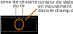
\includegraphics[width=0.5\textwidth]{moteur_visee}
\end{center}

\begin{itemize}
\item[\ding{223}] L'affichage de ce système de visée se fera sur le terminal de l'exécutable. Le curseur de visée se déplacera rapidement de gauche à droite dans le champ de tir (de manière cyclique). L'utilisation de l'instruction système \texttt{system("cls")} permet de \og{}\fg{raffraîchir} le terminal à chaque nouvel affichage du déplacement du curseur.
\item[\ding{223}] Le déclenchement du tir se fera via un appui sur la touche [ESPACE]. La détection de l'appui sera géré grâce à la fonction  \texttt{GetAsyncKeyState} de la librairie \texttt{windows.h} qui permet de \og{}scruter\fg{} de manière \textbf{asynchrone (gestion d'évènements)} l'appui sur une touche spécifique du clavier ([ESPACE], [Echap], etc.).
\item[\ding{223}] La réussite du tir sera conditionnée par cet appui au moment opportun où le curseur de visée entrera dans la \textbf{zone de réussite du tir}.
\item[\ding{223}] Tout ce système sera confié à une fonction \texttt{Assaut} qui renverra un booléen \texttt{true} ou \texttt{false} suivant la réussite où l'échec du tir.
\item[\ding{223}] Les itérations des assauts successifs de chaque vaisseau sera gérée dans le \texttt{main} avec appel de cette fonction \texttt{Assaut} dans la boucle de duel.
\end{itemize}

\textbf{Ce moteur de jeu a été implémenté} et vous est fourni. Il est disponible dans l'archive \fbox{\texttt{moteur\_de\_jeu.zip}} récupérable dans l'onglet \bfcolor{blue}{SAé2 Info2 - Ressources pour le projet d'informatique} sur \ESPACEINFO1. Il contient~:
\begin{itemize}
\item[$\looparrowright$] La librairie des fonctions (nommée \texttt{moteur\_de\_jeu} $\Rightarrow$ fichier d'en-tête \texttt{.h} + fichier source \texttt{.cpp}) implémentant le moteur et notamment la fonction \texttt{Assaut}.
\item[$\looparrowright$]  Un petit programme \texttt{main} d'exemple manipulant le moteur. \textit{Il faudra bien sûr tester ce code puis adapter le programme au cahier des charges du projet.}
\end{itemize}
\end{mycolorbox}

%\vspace{1mm}
%\fbox{\begin{minipage}[l]{\textwidth}
%\itcolor{redCM}{\underline{Quelques aides~:}}
%\begin{itemize}
%%\item[\ding{223}] \textit{Pour générer un entier aléatoire compris entre \texttt{m} et \texttt{n}, il faut utiliser les lignes de code suivantes~:}\\
%%\begin{tt}
%%\#include<time.h> //inclusion de la fonction time()\\
%%\#include<stdlib.h> // inclusion des fonctions rand() et srand()\\
%%// Dans la fonction où vous voulez générer l’entier aléatoire: \\
%%unsigned int alea;\\
%%srand(time(NULL)); //initialisation du générateur \\
%%/* génération d'un entier aléatoire compris \\
%%entre \textit{m} et \textit{n} (avec \textit{m}<\textit{n}) */ \\
%%alea=(rand() \% (\textit{n}-\textit{m}+1))+\textit{m};
%%\end{tt}
%\item[\ding{223}] \textit{Pour générer une pause du programme, il faut utiliser les lignes de code suivantes~:}\\
%\begin{tt}
%\#include<Windows.h> // inclusion de la fonction Sleep()\\
%// Dans la fonction où vous voulez générer une pause: \\
%unsigned int alea;\\
%int cpt;\\
%Sleep(1000*cpt); // pause de cpt secondes
%\end{tt}
%\item[\ding{223}] \textit{Pour éviter d'avoir à taper \texttt{Entrée} après l'appui sur la touche \touche{m} ou \touche{q} :}
%\begin{itemize}
%\item \textit{il faut d'abord, à chaque nouvelle entrée dans la boucle d'assaut, vider le buffer de l'entrée standard \texttt{stdin} (au cas où un ou plusieurs caractères saisis soient encore dans le buffer) avec l'instruction :}\\
%\begin{tt}
%\#include<limits> //inclusion de numeric\_limits \\
%// Dans la fonction où vous voulez générer l’entier aléatoire: \\
%unsigned int alea;\\
%// Demander une saisie + appui sur Entrée pour démarrer un nouvel assaut\\
%int round ;\\
%cout << "Appui sur une touche (n'importe laquelle) + Entrée pour démarrer un nouvel assaut" ;\\
%cin >> round ;\\
%cin.ignore(std::numeric\_limits<std::streamsize>::max(),'$\backslash$n') ;\\
%\end{tt}
%\item \textit{pour la saisie de la "touche d'attaque" à proprement parler, il faut utiliser les lignes de code suivantes :}\\
%\begin{tt}
%\#include<conio.h> //inclusion de la fonction getch()\\
%char touche;\\
%touche = getch(); //récupération de la saisie (à la place de cin >> ...) sans validation par 'Entrée'
%\end{tt}
%\end{itemize}
%\end{itemize}
%\end{minipage}}

\vspace{5mm}
\cboxjalon{\bf Jalon \& Livrable n$^\circ$1 $\Rightarrow$ 01/04/2022}
\begin{mycolorbox}{black}{orange}
Pour ce jalon, vous devrez fournir dans une archive \texttt{ZIP} intitulée\\ \colorbox{yellow}{\texttt{Jalon\_1\_\textit{n$^\circ$binome}.zip}}~:
\begin{itemize}
\item[$\looparrowright$] Votre code fonctionnel et correctement documenté.
\item[$\looparrowright$] Vos journaux de bord, personnel et de groupe, au format numérique PDF.
\end{itemize}
\begin{mycolorbox}{black}{yellow}Si vous n'êtes pas parvenus jusqu'à ce point, vous devez rendre \textbf{votre projet en l'état} à la date prévue.\end{mycolorbox}
\end{mycolorbox}

\addtocounter{quest}{1}
\subsection*{Phase~\thequest : fonctionnalité \texttt{Attaquer}}
\label{phase_attaquer}

\begin{itemize}
\item[$\looparrowright$] On souhaite à présent définir une fonctionnalité \texttt{Attaquer} \og{}appelée par un vaisseau attaquant (l'appelant)\fg{} qui va infliger des dégâts (la cible va donc \textbf{subir des dégâts}) du nombre de sa \textbf{puissance de feu}.\\
\itcolor{redCM}{\underline{Note~:} cette fonctionnalité doit pouvoir utiliser des fonctionnalités déjà implémentées afin de favoriser l'intégrité de votre code.} 
\end{itemize}

\addtocounter{quest}{1}
\subsection*{Phase~\thequest : modification du conteneur \texttt{Vaisseau} et adaptation du duel}
\label{phase_type_vaisseau}

\begin{itemize}
\item[$\looparrowright$] On doit modifier le nom de la fonctionnalité \texttt{Attaquer} en \texttt{AttaquerBasic} qui constituera la \bfcolor{blueTD}{fonctionnalité d'attaque standard} du \texttt{Vaisseau}.
\item[$\looparrowright$] En prévision des phases suivantes, on crée à présent une nouvelle fonctionnalité \texttt{AttaquerSpecial} qui constituera une \bfcolor{blueTD}{méthode d'attaque spécialisée} du \texttt{Vaisseau}. Pour le moment, \bfcolor{blueTD}{conteneur \texttt{Vaisseau} que vous avez implémenté constitue une classe générique de vaisseau}, qui ne possède en soi aucune spécialisation. La fonctionnalité \texttt{AttaquerSpecial} \bfcolor{blueTD}{ne doit donc rien faire hormis afficher un message spécifique}.\\
\itcolor{redCM}{C'est lors des phases suivantes du projet que seront définies des \textbf{classes spécialisées de vaisseaux}, pour lesquelles la fonctionnalité \textnormal{\texttt{AttaquerSpecial}} devra être redéfinie pour permettre de réaliser des actions d'attaque spécifiques.} 
\item[$\looparrowright$] On doit à présent \bfcolor{greenTP}{adapter le programme de duel de vaisseaux} précédemment programmé dans la \bfcolor{greenTP}{phase 2} afin qu'il utilise les nouvelles fonctionnalités \textnormal{\texttt{AttaquerBasic}} et \textnormal{\texttt{AttaquerSpecial}}.\\
\itcolor{redCM}{Il faut alors intégrer un système (de votre choix, aléatoire par exemple) de sélection de l'attaque basique ou de l'attaque spéciale lors d'une itération du duel.}
\end{itemize}

\begin{mycolorbox}{black}{yellow}
\itcolor{redCM}{\underline{Note~:}} cette adaptation doit être implémentée dans un nouveau programme principal, afin de garder trace de l'ancien programme. Vous pouvez créer un nouveau projet \codeblocks et y importer vos librairies de fonctions pour y implémenter un nouveau \texttt{main}.
\end{mycolorbox}

\vspace{5mm}
\cboxjalon{\bf Jalon \& Livrable n$^\circ$2 $\Rightarrow$ 15/04/2022}
\begin{mycolorbox}{black}{orange}
Pour ce jalon, vous devrez fournir dans une archive \texttt{ZIP} intitulée\\ \colorbox{yellow}{\texttt{Jalon\_2\_\textit{n$^\circ$binome}.zip}}~:
\begin{itemize}
\item[$\looparrowright$] Votre code fonctionnel et correctement documenté.
\item[$\looparrowright$] Une première version de la documentation technique du code, au format numérique PDF, contenant a minima les algorithmes des fonctions et programmes développées jusqu'à maintenant.
\item[$\looparrowright$] Vos journaux de bord, personnel et de groupe, au format numérique PDF.
\end{itemize}
\begin{mycolorbox}{black}{yellow}Si vous n'êtes pas parvenus jusqu'à ce point, vous devez rendre \textbf{votre projet en l'état} à la date prévue.\end{mycolorbox}
\end{mycolorbox}

\addtocounter{quest}{1}
\subsection*{Phase~\thequest : définition de 2 conteneurs \og{}spécialisés\fg{} du \texttt{Vaisseau} : \texttt{Croiseur} et \texttt{Chasseur}}
\label{phase_heritage}

On propose de créer des \bfcolor{blueTD}{vaisseaux de classes spécialisées}, c'est-à-dire des vaisseaux qui vont intégrer, en plus des caractéristiques génériques à tout vaisseau, des caractéristiques et fonctionnalités particulières afin d'introduire un peu de variabilité et de personnalisation dans la future constitution de \bfcolor{blueTD}{flottes de vaisseaux}.\\
\bfcolor{redCM}{\underline{Comment faire ?}} Il s'agit de créer des nouveaux conteneurs \og{}spécialisés\fg{} qui doivent \og{}hériter\fg{} des caractéristiques d'un conteneur \texttt{Vaisseau}. Pour éviter de \og{}recopier\fg{} les caractéristiques génériques dans ces nouveaux conteneurs, il faut globalement inclure un conteneur de type \texttt{Vaisseau} comme une caractéristique des conteneurs spécialisés $\Rightarrow$ on aura ainsi \og{}encapsuler\fg{} toutes les caractéristiques génériques et on pourra avoir accès aux fonctionnalités implémentées pour gérer cette caractéristique \texttt{Vaisseau} intégrée au conteneur spécialisé. 

L'objectif de cette phase est donc de~:
\begin{itemize}
\item[$\looparrowright$] créer 2 conteneurs - \itcolor{redCM}{2 nouveaux \textbf{types} de vaisseaux} - \texttt{Croiseur} et \texttt{Chasseur} qui doivent \og{}spécialiser\fg{} le conteneur \texttt{Vaisseau}. Pour le moment ces conteneurs doivent être \bfcolor{blueTD}{vides} hormis la caractéristique \texttt{m\_vaisseau} définissant ce lien \og{}d'héritage\fg{} d'un type \texttt{Vaisseau} dans ces conteneurs.\\
\itcolor{redCM}{D'un point de vue logique, un \textnormal{\texttt{Chasseur}} ou un \textnormal{\texttt{Croiseau}} \textbf{est} un \textnormal{\texttt{Vaisseau}}. D'un point de vue implémentationnel, on le modélise par le fait qu'un \textnormal{\texttt{Chasseur}} ou un \textnormal{\texttt{Croiseau}} \textbf{contient} un \textnormal{\texttt{Vaisseau}}.}
\item[$\looparrowright$] adapter le programme de duel de vaisseaux précédemment programmé dans la \bfcolor{greenTP}{phase 4} afin de tester un duel entre 1 \texttt{Chasseur} et 1 \texttt{Croiseur}.\\
\itcolor{redCM}{L'interaction entre 2 vaisseaux spécialisés doit utiliser les fonctionnalités du type générique \texttt{Vaisseau} - \textnormal{\texttt{AttaquerBasic}} et \textnormal{\texttt{AttaquerSpecial}}. Il faut donc trouver un moyen pour que des vaisseaux spécialisés puissent \og{}appeler\fg{} ces fonctionnalités.}
\end{itemize}

\begin{mycolorbox}{black}{yellow}
\itcolor{redCM}{\underline{Note~:}} une fois de plus, cette adaptation doit être implémentée dans un nouveau programme principal, afin de garder trace des anciens programmes.
\end{mycolorbox}

\addtocounter{quest}{1}
\subsection*{Phase~\thequest : spécialisation du \texttt{Croiseur}}
\label{phase_croiseur}

La spécificité du \texttt{Croiseur} est de disposer d'une \bfcolor{blueTD}{arme spécifique}, le \bfcolor{blueTD}{canon}, matérialisée par 1 nouvelle caractéristique~:
\begin{itemize}
\item[\ding{223}] la puissance de feu du canon.
\end{itemize}

La spécialisation du \texttt{Croiseur} consiste en~:
\begin{itemize}
\item[$\looparrowright$] l'ajout des nouvelles caractéristiques au conteneur \texttt{Croiseur}.
\item[$\looparrowright$] la définition de nouvelles fonctionnalités permettant d'\textbf{affecter} (globalement et individuellement) des valeurs à aux caractéristiques spécifiques d'un croiseur.
\item[$\looparrowright$] la re-définition de la fonctionnalité permettant d'\textbf{afficher} les caractéristiques d'un croiseur.\\
\itcolor{blueTD}{On devra donc afficher aussi bien les nouvelles caractéristiques que les caractéristiques génériques (pour ces derniers on devra ré-utiliser la fonctionnalité \texttt{Afficher} du conteneur \texttt{Vaisseau}).}\\
\itcolor{redCM}{\underline{Note :} d'un point de vie implémentationnel, la re-définition de fonctionnalité va faire appel à la technique de \textbf{surcharge de fonction}. Cette dernière consiste à redéfinir une fonction avec le même nom qu'une autre mais des paramètres d'entrée différents. Ainsi dans notre cas, il s'agit d'adapter la fonctionnalité \textnormal{\texttt{Afficher}} du conteneur \textnormal{\texttt{Vaisseau}} pour que l'\og{}appelant\fg{} soit un \textnormal{\texttt{Croiseur}}.}
\end{itemize}
\begin{mycolorbox}{black}{yellow}
\bfcolor{greenC2}{Il ne faut pas oublier de réaliser des procédures de tests unitaires pour valider chaque nouvel élément ajouté au projet.}
\end{mycolorbox}
\begin{itemize}
\item[$\looparrowright$] la re-définition (sur le même principe que la fonctionnalité \texttt{Afficher}) de la fonctionnalité \texttt{AttaquerSpecial} qui va infliger les dégâts d'un \bfcolor{blueTD}{tir de canon}.\\
\bfcolor{greenTP}{Cette attaque spéciale ne doit avoir qu'1 chance sur 2 de réussir.}
\end{itemize}

\begin{mycolorbox}{black}{yellow}
\itcolor{redCM}{\underline{Note~:}} Si tout est implémenté correctement, le programme de duel entre un croiseur et un chasseur de la phase 5 doit fonctionner correctement sans apporter de modification.
\end{mycolorbox}

\addtocounter{quest}{1}
\subsection*{Phase~\thequest : spécialisation du \texttt{Chasseur}}
\label{phase_escadron}

La spécificité du \texttt{Chasseur} est de disposer d'une \bfcolor{blueTD}{arme spécifique}, les \bfcolor{blueTD}{torpilles}, matérialisée par 2 nouvelles caractéristiques~:
\begin{itemize}
\item[\ding{223}] la puissance de feu des torpilles~;
\item[\ding{223}] le \og{}stock\fg{} disponible de torpilles (qui sera donc décrémenté à chaque utilisation et finira par tomber à zéro).
\end{itemize}

La spécialisation du \texttt{Chasseur} suit les mêmes étapes que la spécialisation du \texttt{Croiseur}. La seule différence sera dans la re-définition de la fonctionnalité \texttt{AttaquerSpecial} \bfcolor{greenTP}{qui aura 100\% de chances de réussite mais sera limitée en nombre d'utilisation, géré par l'une des caractéristiques spéciales du \texttt{Chasseur}.}

\vspace{5mm}
\cboxjalon{\bf Jalon \& Livrable n$^\circ$3 $\Rightarrow$ 06/05/2022}
\begin{mycolorbox}{black}{orange}
Pour ce jalon, vous devrez fournir dans une archive \texttt{ZIP} intitulée\\ \colorbox{yellow}{\texttt{Jalon\_3\_\textit{n$^\circ$binome}.zip}}~:
\begin{itemize}
\item[$\looparrowright$] Votre code fonctionnel et correctement documenté.
\item[$\looparrowright$] Une nouvelle version de la documentation technique du code, au format numérique PDF.
\item[$\looparrowright$] Vos journaux de bord, personnel et de groupe, au format numérique PDF.
\end{itemize}
\begin{mycolorbox}{black}{yellow}Si vous n'êtes pas parvenus jusqu'à ce point, vous devez rendre \textbf{votre projet en l'état} à la date prévue.\end{mycolorbox}
\end{mycolorbox}

\addtocounter{quest}{1}
\subsection*{Phase~\thequest : consolidation du moteur du programme}
\label{phase_surcharge}

Pour le moment, les programmes de duel entre 2 vaisseaux sont conçus spécifiquement pour gérer un combat entre 2 vaisseaux dont on connait la classe~:
\begin{itemize}
\item[\ding{223}] Un \texttt{Vaisseau} contre un \texttt{Vaisseau}~;
\item[\ding{223}] Un \texttt{Croiseur} contre un \texttt{Chasseur}~;
\end{itemize}

On souhaite pouvoir généraliser le programme de duel pour que son \textbf{algorithme principal} soit le même quels que soient les 2 vaisseaux \og{}duellistes\fg{}, autrement dit quels que soient les 2 vaisseaux déclarés dans le \textbf{lexique principal}.

\begin{itemize}
\item[$\looparrowright$] Pour ce faire, il faut rendre \textbf{génériques} les appels aux fonctionnalités \texttt{AttaquerBasic} et \texttt{AttaquerSpecial} pour que la compilation du programme \og{}détecte automatiquement\fg{} les classes de vaisseaux antagonistes~:
\begin{itemize}
\item[\ding{223}] Un \texttt{Vaisseau} attaque un \texttt{Croiseur}~;
\item[\ding{223}] Un \texttt{Croiseur} attaque un \texttt{Vaisseau}~;
\item[\ding{223}] Un \texttt{Chasseur} attaque un \texttt{Chasseur}~;
\item[\ding{223}] Un \texttt{Croiseur} attaque un \texttt{Croiseur}~;
\item[\ding{223}] etc.
\end{itemize}
On va procéder en \bfcolor{redCM}{surchargeant} ces fonctionnalités en autant de versions que de cas possibles.
\item[$\looparrowright$] On peut alors générer autant d'exécutables du programme de duel en ne changeant avant compilation que la déclaration des 2 vaisseaux antagonistes.
\end{itemize}

\cboxjalon{\bf Jalon \& Livrable n$^\circ$4 $\Rightarrow$ 24/05/2022}

\cboxjalon{\bf OBJECTIF MINIMAL DU PROJET}

\begin{mycolorbox}{black}{orange}
Il \underline{faut} arriver à rendre ce code fonctionnel, et tout doit être finalisé pour le rendu final du projet.

Pour ce jalon, vous devrez fournir dans une archive \texttt{ZIP} intitulée\\ \colorbox{yellow}{\texttt{Jalon\_4\_\textit{n$^\circ$binome}.zip}}~:
\begin{itemize}
\item[$\looparrowright$] Votre code fonctionnel et correctement documenté.
\item[$\looparrowright$] La documentation technique du code, au format numérique PDF.
\item[$\looparrowright$] Vos journaux de bord, personnel et de groupe, au format numérique PDF.
\end{itemize}
\begin{mycolorbox}{black}{yellow}Si vous n'êtes pas parvenus jusqu'à ce point, vous devez rendre \textbf{votre projet en l'état} à la date prévue.\end{mycolorbox}
\end{mycolorbox}

\addtocounter{quest}{1}
\subsection*{Phase~\thequest : création d'un conteneur \texttt{Flotte}}
\label{phase_flotte}

\begin{itemize}
\item[$\looparrowright$] L'objectif final est de pouvoir gérer une \textbf{bataille globale entre 2 flottes de vaisseaux}. Pour ce faire, on propose de créer un conteneur \texttt{Flotte} qui contiendra plusieurs vaisseaux~: 
\begin{itemize}
\item[\ding{223}] 1 \texttt{Croiseur}~;
\item[\ding{223}] 2 \texttt{Chasseur}~;
\item[\ding{223}] 3 \texttt{Vaisseau}.
\itcolor{redCM}{\underline{Note :} ces vaisseaux doivent être regroupés par type, autrement dit une caractéristique du conteneur \texttt{Flotte} correspond à un groupement de vaisseaux d'un certain type $\Rightarrow$ \textbf{le type approprié est donc à déterminer}.}
\end{itemize}
\item[$\looparrowright$] Une instance de \texttt{Flotte} doit disposer des fonctionnalités suivantes~:
\begin{itemize}
\item[\ding{223}] 1 fonctionnalité permettant d'\textbf{afficher} l'état de la \texttt{Flotte} : informations sur chaque \texttt{Vaisseau}. Cette fonctionnalité \bfcolor{blueTD}{doit entre autres appeler les fonctionnalités \texttt{Afficher} de chaque \texttt{Vaisseau}, \texttt{Croiseur} et \texttt{Chasseur} de la flotte}.
\item[\ding{223}] plusieurs fonctionnalités (1 par type de vaisseau) permettant de \bfcolor{blueTD}{modifier les caractéristiques d'un \texttt{Vaisseau}, \texttt{Croiseur} ou \texttt{Chasseur} de la flotte}.\\
\itcolor{redCM}{\underline{Note :} la désignation d'un \textnormal{\tt Vaisseau}, \textnormal{\tt Croiseur} ou \textnormal{\tt Chasseur} au sein de la \textnormal{\tt Flotte} doit être géré par un \textbf{numéro d'ordre}~:
\begin{itemize}
\item $\{1, 2, 3\}$ pour l'un des 3 \textnormal{\tt Vaisseau}.
\item $\{4, 5\}$ pour l'un des 2 \textnormal{\tt Chasseur}.
\item $\{6\}$ pour le \textnormal{\tt Croiseur}.
\end{itemize}
Ce \textbf{numéro d'ordre} (type \textnormal{\tt int}) sera un des paramètres d'entrée des fonctionnalités \textbf{d'affectation}, afin de désigner le bon vaisseau.}
\item[\ding{223}] 1 fonctionnalité qui renvoie \texttt{VRAI} si l'ensemble des vaisseaux de la flotte sont détruits, et \texttt{FAUX} sinon.
\end{itemize}
\item[$\looparrowright$] Ce nouveau conteneur étant assez conséquent, un soin particulier doit être porté aux \bfcolor{greenC2}{procédures de tests unitaires} afin de valider rigoureusement le bon fonctionnement de ce conteneur.\\
\end{itemize}

\addtocounter{quest}{1}
\subsection*{Phase~\thequest : l'ultime bataille}
\label{phase_bataille1}

\begin{itemize}
\item[$\looparrowright$] Nous voici enfin à l'objectif final de ce projet~: \textbf{la mise en place d'un \og{}jeu de combat\fg{} entre 2 \texttt{Flotte} au tour par tour}. Voici l'algorithme simplifié à coder dans votre programme principal~:

\begin{algorithme}
Création et initialisation des flottes.\\
\textbf{Répéter}
\begin{equation*}
\left| \begin{array}{l}
\hspace{5mm}\text{Définir le tour du joueur courant.} \\
\hspace{5mm}\text{Afficher l'état des flottes.} \\
\hspace{5mm}\text{Choisir le vaisseau attaquant puis le vaisseau ciblé.} \\
\hspace{5mm}\text{Choisir le type d'attaque.} \\
\hspace{5mm}\text{Résoudre l'attaque.} \\
\hspace{2mm}\text{\bf Jusqu'à (\textit{destruction d'une des 2 flottes})}
\end{array} \right.
\end{equation*}
\textbf{FinRépéter}

\textbf{Afficher le vainqueur.}

\end{algorithme}

\item[$\looparrowright$] La mise en œuvre de requiert d'ajouter au conteneur \texttt{Flotte} une fonctionnalité \texttt{ChoixVaisseau} qui doit récupérer (en entrée/sortie) un pointeur vers le \texttt{Vaisseau}, \texttt{Croiseur} ou \texttt{Chasseur} en fonction du \textbf{numéro d'ordre} du vaisseau dans la flotte donné en entrée.\\
\bfcolor{redCM}{Il faudra créer 3 surcharges de cette fonctionnalité pour qu'elle puisse récupérer, suivant le cas, un pointeur vers l'un des 3 types de \texttt{Vaisseau}.}
%\itcolor{redCM}{\underline{Note :} la désignation d'un \textnormal{\tt Vaisseau}, \textnormal{\tt Croiseur} ou \textnormal{\tt Chasseur} au sein de la \texttt{Flotte} sera gérée par un \bfcolor{red}{numéro d'ordre}~:
%\begin{itemize}
%\item $\{1, 2, 3\}$ pour l'un des 3 \textnormal{\tt Vaisseau}.
%\item $\{4, 5\}$ pour l'un des 2 \textnormal{\tt Chasseur}.
%\item $\{6\}$ pour le \textnormal{\tt Croiseur}.
%\end{itemize}
%Ce \bfcolor{red}{numéro d'ordre} (type \textnormal{\tt int}) sera le paramètre d'entrée de la fonctionnalité \textnormal{\tt ChoixVaisseau}. Dans le programme principal, il faudra donc demander à l'utilisateur de choisir le numéro du vaisseau de la \textnormal{\tt Flotte} et récupérer le "bon" pointeur.}
\item[$\looparrowright$] Dans un premier temps, on devra \bfcolor{greenC2}{tester le système de choix de vaisseau} en proposant une version  du programme de duel permettant définir 2 flottes et d'organiser un duel entre 2 vaisseaux de ces flottes.
\item[$\looparrowright$] Enfin, on mettra en place tout \bfcolor{blueTD}{le programme du jeu}.
\end{itemize}

\cboxjalon{\bf Jalon \& Livrable n$^\circ$5 $\Rightarrow$ 10/06/2022}

\cboxjalon{\bf OBJECTIF FINAL DU PROJET}

\begin{mycolorbox}{black}{orange}
Si vous arrivez jusqu'à ce jalon et que votre programme est totalement opérationnel (donc \og{}jouable\fg{}), \textbf{vous êtes les rois du monde}~!

Pour ce jalon, vous devrez fournir dans une archive \texttt{ZIP} intitulée\\ \colorbox{yellow}{\texttt{Jalon\_5\_\textit{n$^\circ$binome}.zip}}~:
\begin{itemize}
\item[$\looparrowright$] Votre code fonctionnel et correctement documenté.
\item[$\looparrowright$] La documentation technique du code, au format numérique PDF.
\item[$\looparrowright$] Vos journaux de bord, personnel et de groupe, au format numérique PDF.
\item[$\looparrowright$] \colorbox{yellow}{\bfcolor{black}{Une soutenance de votre projet sous forme d'une vidéo de 15 minutes.}} \itcolor{black}{Les modalités seront explicitées plus tard.}
\end{itemize}
\begin{mycolorbox}{black}{yellow}Si vous n'êtes pas parvenus jusqu'à ce point, vous devez rendre \textbf{votre projet en l'état} à la date prévue.\end{mycolorbox}
\end{mycolorbox}

\addtocounter{quest}{1}
\subsection*{Phase~\thequest : quelques objectifs bonus (facultatifs)}
\label{phase_objectifs_bonus}

\begin{itemize}
\item[$\looparrowright$] On propose dans cette phase quelques pistes d'exploration permettant de profiter de ce projet pour  \bfcolor{redCM}{faire monter vos compétences de programmeurs}.
\item[$\looparrowright$] Ces \bfcolor{redCM}{objectifs} sont \bfcolor{redCM}{facultatifs} mais feront l'objet d'une \bfcolor{redCM}{bonification} dans l'évaluation de votre projet~: ils sont à explorer en totale liberté et autonomie.\\ \bfcolor{blueTD}{Vous êtes également libres d'explorer d'autres pistes suivant où vous porte votre curiosité \og{}informatique\fg{}.}\\
\itcolor{redCM}{\bf Vous devrez vous-mêmes rechercher les ressources (tutoriels, documentations) pour vous aider à comprendre l'objectif et le mettre en œuvre dans votre programme.}
\item[$\looparrowright$] Voici la liste (non exhaustive) des objectifs proposés~:
\end{itemize}

\begin{mycolorbox}{black}{yellow}
\begin{itemize}
\item[\ding{223}] \bfcolor{black}{Étudier la possibilité de créer des flottes personnalisées (nombre de vaisseaux, choix des types de vaisseaux) en utilisant notamment le principe d'allocation dynamique de mémoire.}
\item[\ding{223}] \bfcolor{black}{Explorer la notion de \og{}pointeur générique\fg{} (\textit{void pointer} en anglais) \texttt{void*} pour faciliter la gestion de choix de vaisseaux dans un conteneur \texttt{Flotte} (en évitant trop de surcharges).}
\item[\ding{223}] \bfcolor{black}{Explorer la gestion de fichiers (création/ouverture/lecture/écriture).} Par exemple~:
\begin{itemize}
\item écrire dans un fichier une partie de la sortie d'exécution (par exemple l'état de la partie à chaque tour)
\item inventorier dans un ou plusieurs fichiers toutes les \og{}parties jouées\fg{} (à chaque exécution du programme) en précisant (suggestion) : le nom des joueurs, la date de la partie, sa durée, le nombre de tours de jeu, le vainqueur, etc.
\item écrire dans des fichiers au préalable les caractéristiques de chaque vaisseau d'une flotte, puis initialiser les flottes en allant lire ces caractéristiques dans les fichiers.
\end{itemize}
\item[\ding{223}] \bfcolor{black}{Améliorer le moteur de jeu gérant la visée et le tir.} Par exemple~:
\begin{itemize}
\item proposer un affichage graphique plus élégant du système de visée mais toujours en mode \og{}terminal\fg{}~;
\item \bfcolor{black}{aller plus loin en utilisant d'autres librairies/API (en langage C) plus graphiques pour gérer ce moteur.} Par exemple~:
\begin{itemize}
\item l'API \bfcolor{redCM}{ncurses}~: [\url{https://fr.wikipedia.org/wiki/Ncurses}]~; [\url{https://invisible-island.net/ncurses/}].
\item la \bfcolor{redCM}{Simple DirectMedia Layer (SDL)}~: [\url{https://fr.wikipedia.org/wiki/Simple_DirectMedia_Layer}] ; [\url{https://zestedesavoir.com/tutoriels/1014/utiliser-la-sdl-en-langage-c/la-sdl/}] ; [\url{https://www.libsdl.org/}].
\end{itemize}
\end{itemize}
\item[\ding{223}] Explorer l'utilisation d'un outil de versionnage de code tel que \bfcolor{redCM}{Git}, notamment via la plateforme (type \og{}cloud\fg{}) dédiée \bfcolor{redCM}{GitHub}~: [\url{https://git-scm.com/}]~;[\url{https://github.com/}].
\item[\ding{223}] Explorer l'utilisation d'un outil de génération de documentation à partir des commentaires d'un code tel que \bfcolor{redCM}{Doxygen}~: [\url{https://www.doxygen.nl/index.html}].
\item[\ding{223}] \bfcolor{black}{N'hésitez pas à explorer d'autres pistes qui vous intéressent ou à proposer d'autres améliorations du programme (autre système de jeu, enrichissement des types de vaisseaux, etc.).} 
\end{itemize}
\end{mycolorbox}

\begin{mycolorbox}{black}{yellow}
\large \bf Certains de ces objectifs annexes peuvent être traités en parallèle de l'élaboration du projet. Vous pouvez organiser votre travail d'équipe pour que certains d'entre vous se dédient à ces tâches. \bfcolor{redCM}{Quoi qu'il en soit, les phases 1 à 10 restant les objectifs prioritaires et obligatoires.}
\end{mycolorbox}


\end{document}

